%%---------------------------------------------------------------------------%%
%% dbs.tex
%% Thomas M. Evans
%% $Id$
%%---------------------------------------------------------------------------%%
\documentclass[11pt]{../tex/rnote}
\usepackage[centertags]{amsmath}
\usepackage{amssymb,amsthm,graphicx}
\usepackage[mathcal]{euscript}
\usepackage{tabularx}
\usepackage{cite}
\usepackage{c++}
\usepackage{tmadd,tmath}
\usepackage{stl}
\usepackage{draco_bs}
\usepackage{alltt}
\usepackage{makeidx}

%%---------------------------------------------------------------------------%%
%% DEFINE SPECIFIC ENVIRONMENTS HERE
%%---------------------------------------------------------------------------%%

\newcommand{\dsxx}{\pkg{ds\raisebox{.2ex}{\scriptsize++}}}
\newcommand{\imc}{\pkg{imc}}

\newcommand{\draco}{\sys{Draco}}

\newcommand{\autoconf}{\soft{Autoconf}}
\newcommand{\automake}{\soft{Automake}}
\newcommand{\make}{\soft{Make}}

\makeindex

%%---------------------------------------------------------------------------%%
%% BEGIN DOCUMENT
%%---------------------------------------------------------------------------%%

\begin{document}

%%---------------------------------------------------------------------------%%
%% OPTIONS FOR NOTE
%%---------------------------------------------------------------------------%%

\toms{Distribution}
%\toms{Joe Sixpak/XTM, MS B226}
\refno{X-6:97-??? (U)}
\subject{The Draco Build System}

%-------NO CHANGES
\divisionname{Computer and Computational Sciences}
\groupname{CCS--4:Transport Methods Group}
\fromms{Thomas M. Evans/CCS-4 D409}
\phone{(505)665--3677}
\originator{tme}
\typist{tme}
\date{\today}
%-------NO CHANGES

%-------OPTIONS
%\reference{NPB Star Reimbursable Project}
%\thru{P. D. Soran, XTM, MS B226}
%\enc{list}      
%\attachments{list}
%\cy{list}
%\encas
%\attachmentas
%\attachmentsas 
%-------OPTIONS

%%---------------------------------------------------------------------------%%
%% DISTRIBUTION LIST
%%---------------------------------------------------------------------------%%

\distribution {}

%%---------------------------------------------------------------------------%%
%% BEGIN NOTE
%%---------------------------------------------------------------------------%%

\opening

\begin{abstract}
  
  We present an updated build system for the \draco\ component
  library.  The \draco\ Build System (DBS) \index{Draco Build System}
  is designed to facilitate both development and usage on multiple
  platforms.  The DBS complies with the GNU Coding Standards for
  software packages.  It has been designed according to the following
  list of requirements:
  \begin{enumerate}
  \item support for simultaneous, multiple configurations;
  \item support for \C++ on all ASCI platforms;
  \item automated unit and regression testing;
  \item the ability to support multiple code projects;
  \item support for external vendors;
  \item support for multiple languages;
  \item extensibility;
  \item low-cost on developers to add new packages, code, and tests; 
  \item compliance with the GNU coding standard \cite{gnu}.
  \end{enumerate}
  These requirements are largely met by the DBS.  In fact, the DBS is
  being used as the build system for 4 CCS--4 projects.
  
  The build system uses four GNU development tools, \autoconf,
  \automake, and \make. These tools are all freely available from the
  Free Software Foundation.

\end{abstract}

%%---------------------------------------------------------------------------%%
%% INCLUDES
%%---------------------------------------------------------------------------%%

%%---------------------------------------------------------------------------%%
%% intro.tex
%% introduction of Draco build system manual
%%---------------------------------------------------------------------------%%

\chapter{Introduction}

In this chapter we will examine the %purpose for redesigning the
design contraints of the \draco\ build system (DBS).  We will
introduce some definitions of terms and typographical conventions that
will be employed throughout the text.  Additionally, the organization
of the manual will be described.  For those who wish to get started
right away, \S~\ref{sec:quick} tells how to get up and moving without
working through the manual.  A detailed developer manual is processed
with \soft{Doxygen}~\cite{doxygen} and is maintained with the
\draco\ source code.

%%---------------------------------------------------------------------------%%

\section{Purpose}
\label{sec:purpose}

The purpose of this document is to describe the \draco\ build system.
Specifically, we will show both users and \draco\ developers how to: 
\begin{itemize}
\item configure \draco\ for different platforms and options;
\item compile \draco\ components;
\item compile and link programs that use \draco;
\item add packages to \draco;
\item add new support options to \draco.
\end{itemize}
Thus, this manual is an invaluable reference to those who work in, or
with, \draco.

As a review, we restate the \draco\ mission statement~\cite{rn98046}:
\begin{quote}
  \slshape \draco\ is a comprehensive, readiation transport framework
  that provides key, reusable components for serial and parallel,
  computational physics codes.
\end{quote}
To meet these requirements \draco\ uses modern software engineering
concepts including object-oriented/\-generic design, multi-environment
build systems, and service libraries based on levelized component
designs.  The build system described in this manual allows \draco\ to
satisfy its mission statement and enforces the concept of levelized
component design.

The \draco\ build system has been carefully designed.  In particular,
we had several requirements that the build system should satisfy.
These requirements are:
\begin{itemize}
\item support for simultaneous multiple configurations;
\item support for multiple languages, particularly \cpp, \cc, and
  \python on all ASC platforms;
%\item support for \dejagnu\ and regression testing;
\item on-demand and automated unit and regression testing;
\item the ability to support multiple code projects;
\item support for external vendors;
\item support for multiple languages;
\item extensibility;
\item low-cost on developers to add new packages, code, and tests; 
\item compliance with the GNU coding standard \cite{gnu} \index{GNU
    Coding Standard}.
\end{itemize}
This last requirement has evolved a somewhat as the supported
platforms and build systems scope has grown to include XCode and
Eclipse on non-Linux platforms.  The use of the CMake suite of tools
preculdes the use of GNU autotools \index{GNU autotools},
\autoconf\ and \automake~\cite{autoconf}.  
It also precludes the use of \make~\cite{gmake} for non-Makefile based
build projects (e.g.: XCode, Eclipse). More detail will be given in
Chap.~\ref{chap:model}. 

%%---------------------------------------------------------------------------%%

\section{Definitions and Conventions}

Before continuing we shall clarify the terminology and typeface
conventions that will be employed throughout the remainder of this
manual.  The definitions that we use here are for convenience.  They
are not to be interpreted as an ``universal standard.''  They are
simply used to make sure that the concepts illucidated within this
manual have a common point of reference.

A \latin{product} is anything that is produced from a source code
tree~\cite{ja94}.  A \latin{system} is a code, or a group of codes,
that persist over time~\cite{tn98}.  A \latin{project} is an
undertaking that has a definite beginning and ending date, and it
produces a product.  A \latin{package} is one component of a system
(package and components are used interchangeably).  Packages normally
reside in a single directory in the source code tree; although, that
directory may have subdirectories.  However, packages are sometimes
used to refer to larger units.  For example, a code package may be a
system that contains many components.  In this case, package has macro
(system level) and micro (system-component level) connotations.

Table ~\ref{tab:tfaces} show the typefaces that we will employ
\begin{table}
  \begin{center}
    \caption{Typefaces used throughout the text.}
    \label{tab:tfaces}
    \begin{tabular}{c}\hline\hline
      \sys{code systems} (\draco) \\
      \pkg{packages} (\dsxx) \\
      \comp{files} (\comp{Makefile}) \\
      \vble{variables} (\comp{draco/src/\vble{pkg}/}) \\
      \soft{software programs} (\gmake) \\
      \lang{languages} (\cpp) \\ \hline\hline
    \end{tabular}
  \end{center}
\end{table}
throughout the text to better distinguish certain elements.  In
general, anything that exists on a computer screen (directory trees,
files, etc) is typefaced using \comp{typewriter} font.  Files are
distinguished in the standard UNIX way by appending the following
symbols after the name, \comp{*} for executables, \comp{/} for
directories, and @ for links.  Computer screen prompts are represented
by the \comp{\$} symbol.

%%---------------------------------------------------------------------------%%
\section{DBS Support and Procurement}

Questions about procuring a copy of the DBS or its use can be
directed to:
\begin{center}
  \begin{tabular}{llc}\hline\hline
    \multicolumn{1}{c}{Name} & \multicolumn{1}{c}{Email} &
    Group \\ \hline
%    Tom Evans & tme@lanl.gov & CCS--4 \\
    Kelly Thompson & kgt@lanl.gov     & CCS--2 \\ \hline\hline
    Jae Chang      & jhchang@lanl.gov & CCS--2 \\ \hline\hline
  \end{tabular}
\end{center}
Additional information is available on the \draco\ \soft{TeamForge}
site, \comp{https://tf.lanl.gov/draco}.

%%---------------------------------------------------------------------------%%

\section{Manual Organization}

This manual is written for three basic groups: (a) \draco\ users, (b)
\draco\ package developers, and (c) \draco\ system developers. The
manual is organized around these three groups. There is an additional
group consisting of developers who plan to use \draco\ as a model for
their own code systems.  For this group the entire \draco\ Build
System Manual is of interest.

The \draco\ users group consists of clients who use \draco\ components
in some form.  The primary interest of this group is configuring and
compiling \draco\ so that it meets their product's needs.  The
relationship between this group and \draco\ can be very close (XTM
code teams) or very distant (XCI code teams).

The \draco\ package developers group contains people who write
packages in \draco.  The primary interest of this group is
configuring, compiling, and adding new packages to \draco.  The final
group, the \draco\ system developers group, are those who maintain the
\draco\ infrastructure, including the build system.  This group is
concerned with maintaining the integrity and stability of \draco\ as a
whole unit. Tables~\ref{tab:draco_package} and \ref{tab:draco_system}
%%% GROUP ROSTERS
\begin{table}
  \begin{center}
    \caption{Roster of the \draco\ package developer group.}
    \label{tab:draco_package}
    \begin{tabular}{llc}\hline\hline
      \multicolumn{1}{c}{Name} & \multicolumn{1}{c}{Email} &
      Group \\ \hline
      John McGhee$^{\ast}$ & mcghee@lanl.gov & XTM \\
      Tom Evans & tme@lanl.gov & XTM \\
      Mark Gray & gray@lanl.gov & XTM \\
      Rob Lowrie & lowrie@lanl.gov & XTM \\
      Shawn Pautz & pautz@lanl.gov & XTM \\ 
      Randy Roberts & rsqrd@lanl.gov & XTM \\
      Todd Urbatsch & tmonster@lanl.gov & XTM \\ \hline\hline
      \multicolumn{3}{l}{$^{\ast}$\draco\ project leader.} \\
    \end{tabular}
  \end{center}
\end{table}
\begin{table}
  \begin{center}
    \caption{Roster of the \draco\ systems developer group.}
    \label{tab:draco_system}
    \begin{tabular}{llc}\hline\hline
      \multicolumn{1}{c}{Name} & \multicolumn{1}{c}{Email} &
      Group \\ \hline
      Tom Evans & tme@lanl.gov & XTM \\
      Randy Roberts & rsqrd@lanl.gov & XTM \\ \hline\hline
    \end{tabular}
  \end{center}
\end{table}
%%% END GROUP ROSTERS
gives a current list of the \draco\ package and system developers.

Table~\ref{tab:layout} lists the groups that each chapter targets.
\begin{table}
  \begin{center}
    \caption{The target groups for each chapter.  Group (a) are the
      \draco\ users; Group (b) are the \draco\ package developers, and 
      Group(c) are the \draco\ system developers.}
    \label{tab:layout}
    \begin{tabular}{ccc}\hline\hline
      Chapter & Primary Target Group & Secondary Target Groups
      \\ \hline 
      \ref{chap:model} & (a), (b), (c) & (a), (b), (c) \\ 
      \ref{chap:compile} & (a), (b) & (c) \\ 
      \ref{chap:extern} & (a) & (b) \\
      \ref{chap:adding} & (b) & (c) \\ 
      \ref{chap:extend} & (c) & (b) \\ \hline \hline
    \end{tabular}
  \end{center}
\end{table}
Chapter~\ref{chap:model} gives an overview of the \draco\ source tree
and build system. A complete listing of the \draco\ source tree is
included in this chapter. This chapter is useful for all three groups
that are associated with \draco.

Chapter~\ref{chap:compile} describes how to configure and compile the
\draco\ system.  Included in this chapter are detailed descriptions of
all the \draco\ configure options. Chapter~\ref{chap:extern} shows how
to emulate the \draco\ build model and functionality in external code
systems that use \draco.  This chapter is geared to code teams that
heavily use \draco, and, thus, they may gain advantages by using the
\draco\ build model. These chapters target the \draco\ users and
\draco\ package developers groups.

Chapter~\ref{chap:adding} shows how to add new component packages to
\draco.  In this chapter detailed instructions are given that show how
to add a new package directory, test directory, and, to a lesser
extent, build options.  The intended audience for this chapter is the
\draco\ package developers, and, to a lesser extent, \draco\ system
developers will use this material.

Finally, Chap.~\ref{chap:extend} shows how to extend the \draco\ build 
system.  This chapter focuses on adding new configure options and new
language support.  In general, this chapter shows how the \gmake\ and
\autoconf\ files are used and work.  This chapter is primarily intended
for \draco\ system developers; however, some content in this chapter
is necessary for \draco\ package developers.

%%---------------------------------------------------------------------------%%

\section{Quick Start}
\label{sec:quick}

Many \draco\ users will undoubtedly be familiar with \autoconf\ and
\gmake. These users can progress directly to \S~\ref{sec:examples} for 
examples on configuring and building \draco. 


%%---------------------------------------------------------------------------%%
%% model.tex 
%% description of the draco component library and overview of the build system
%% ---------------------------------------------------------------------------%%

\chapter{The Draco Model}
\label{chap:model}

This chapter presents an overview of the \draco\ build model and
source.  We present, in detail, the requirements for the \draco\ build
system in \S~\ref{sec:build_sys_req}.  Because the \draco\ build model
has been designed to conform to the GNU coding standard, a brief
summary of GNU requirements is given in \S~\ref{sec:gnu_build_model}.
Finally, this chapter concludes with a description of the \draco\ 
source tree and files that are created during configuring and
building.

This section gives an overview of the DBS architecture.  As mentioned
in \S~\ref{sec:intro}, the DBS is a GNU-based \autoconf/\make system.
In this section we will describe the organization of files that make
up the DBS.

%%---------------------------------------------------------------------------%%

\section{Overview of Draco}
\label{sec:overview_of_draco}

Documentation describing the purpose and capabilities of packages
within \draco\ is beyond the scope of this text.  However, a brief
summary of \draco\ is pertinent to this discussion.  \draco\ is a
component library for computational radiation transport.  \draco\ is
primarily a \cpp\ library; however, other language support is not
precluded in \draco.  In particular, \draco\ has plans to support
automatic type-interfacing between \cpp\ and \fortran~\cite{gr99}.
Additionally, we plan to incorporate a generalized interface for
problem input specifications using \python\ extensions.

The products of \draco\ are individual component (package) libraries
that provide reusable services geared towards radiation transport
applications.  For example, \draco\ provides radiation physics, Monte
Carlo, and deterministic solver packages that are templated on Mesh
Types (MT).  In addition to explicit radiation transport components,
\draco\ provides several service packages including \dsxx, a data
structures library that contains numeric containers, smart pointers,
and assertions, and \cfour, a communications library, among others.

The fundamental principle guiding code design in \draco\ is templating
on Mesh Types (MT).  Thus, the libraries in \draco\ will work with any
code that provides a MT with the proper services.  This allows highly
efficient implementations of various meshes to be included in generic
radiation transport packages.  

\draco\ is designed using object-oriented~\cite{me97} and generic
programming~\cite{au99} philosophies.  Foremost among these notions
are levelized design, Design-by-Contract$^{\text{\footnotesize TM}}$,
and the generic concept-model idea.  Other software engineering
methods are employed for quality control including regression testing,
automatic documentation, code profiling, and design and code reviews.

%%---------------------------------------------------------------------------%%

\section{Overview of the Draco Build Model}
\label{sec:overview_draco}

\subsection{Software Requirements}

The \draco\ build system is designed according to the GNU coding
standard.  Accordingly, the following GNU tools are required to
configure and build \draco: \autoconf~\cite{autoconf},
\gmake~\cite{gmake}, \gmfour~\cite{m4}.  In addition, \draco\ version
control is performed by \cvs~\cite{cvs}.  For \draco\ users,
\autoconf\ is not a necessity as the configure scripts will be
distributed with \draco\ releases.

Additional software is used for performing quality control.
Regression testing is handled by \dejagnu~\cite{dejagnu}.  Bugs are
tracked using \gnats~\cite{gnats}.  In addition, an archived email
list is available to submit design plans and discussion between team
members.  Also, \purify~\cite{purify} plays an important part of the
quality control process.  The build system supports linking code for
processing through \purify\ on all platforms.

The \draco\ build system contains support for multiple language
environments.  However, the primary language in use at present is ANSI
Standard \cpp~\cite{ansi:cpp}.  Therefore, any ANSI-compatible \cpp\ 
compiler will compile \draco.  Unfortunately, the Kuck and Associates
\cpp\ compiler, \soft{KCC}~\cite{kai}, is the only ANSI Standard
compatible compiler on the market today.  Thus, \soft{KCC} is required
to compile \draco\ in its entirety. \soft{KCC} is available on all
platforms of interest to Los Alamos National Laboratory and the
Accelerated Strategic Computing Initiative (ASCI).  Currently, there
is no \fortran\ code in \draco; although, we expect that to change in
the future.  Additional languages required by \draco\ are \python\,
\lang{PERL}, and \lang{Tcl/TK}.  \draco\ expects these scripting
languages to be located in standard places (\comp{/usr/local}), and
the build system checks for this.  \TeX\ and \LaTeX\ are also
necessary for compiling the documentation that comes with \draco.

With the exception of \soft{KCC} and \purify, all of the
aforementioned software products are freely available and should be
installed on any standard UNIX system.  Note that \purify\ is mainly a
development tool and is not required to configure, build, or use
\draco.  The remaining software products are required.  The build
system checks for the presence of each of these products; thus, as
long as the software is in the user's path, the configuration will
succeed.  Finally, \draco\ utilizes a number of vendor libraries,
depending upon configuration, that must be installed on the system in
which \draco\ resides.  Detail on these packages and their
configuration options is given in Chap.~\ref{chap:compile}.

\subsection{Build System Requirements}
\label{sec:build_sys_req}

In \S~\ref{sec:purpose} the requirements that guided the development
of the \draco\ build system were summarized.  In this section, we
shall take an expanded look at the complete list of requirements.  The
list of requirements for the \draco\ build system is:
\begin{enumerate}
\item support for simultaneous, multiple configurations;
\item support for \cpp\ explicit template instantiation;
\item support for multiple languages;
\item support for \dejagnu\ and regression testing;
\item support for \purify;
\item compliance with the GNU coding standard.
\end{enumerate}
We will analyze each of these requirements in turn.  First, from a
development standpoint, having multiple configurations at the same
time is a must.  This feature is required because certain tools work
better on certain platforms.  Additionally, certain tools work better
in certain environments.  For example, we often require both scalar
and parallel versions of the code for profiling and testing.  The
\draco\ build systems allow each configuration, and the products it
produces, to exist in a unique directory.  Thus, builds are not
performed in the source code tree; they are done in a user-specified
directory.  More detail is given on multiple configurations and builds 
in \S~\ref{sec:draco_src_tree} and Chap.~\ref{chap:compile}.

A guiding principle of the \draco\ build system is explicit template
instantiation.  We have found that this provides a much more robust
and efficient build system then if the compiler is allowed to
instantiate template classes and functions.  The essence of explicit
instantiation is that the package developer determines what classes
are templated, not the compiler.  \draco\ does not implicitly
instantiate template classes and functions.  \draco\ has rules on how
template classes and functions are explicitly instantiated.  These are
listed in Chap.~\ref{chap:adding}.  Additional information for clients
that use \draco\ class and function templates is listed in
\S~\ref{sec:using}.

\draco\ is not a single language system.  Although \draco\ is
presently composed of \cpp\ code, we expect multiple languages
(\fortran) to be supported for interfacing and numerical
optimization.  The \draco\ build system is general and is not
restricted to single language support.  Supporting multiple languages
is an essential requirement because \draco\ customers utilize many
frameworks and languages.

The next two requirements are aimed at \draco\ system and package
developers and are essential for good quality software.  The \draco\ 
build system must support \dejagnu.  Regression testing is an
important part of the \draco\ quality assurance program.  The daily
testing of \draco\ components, using \dejagnu, ensures that commits to
one part of the library do not adversely affect other components.  In
addition, \purify\ support is necessary to diagnose all \draco\ 
components.

The final requirement is also the most comprehensive; the \draco\ 
build system should conform to the GNU Coding Standard as specified in
Ref.~\cite{gnu}.  We choose to standardize on the GNU model because of 
the success and familiarity with GNU products in the marketplace.  By
formalizing our build model on an accepted standard, we reduce the
overhead associated with maintaining the system, and all of the
software that has been developed by GNU over the years is easily
applicable to \draco.  In addition, the GNU standard is perfectly
suited to the platforms that are in use by our customers.  Finally, by 
using the GNU standard, we gain the benefit of using GNU's
documentation as our own.  A summary of the pertinent parts of the GNU 
standard is given in \S~\ref{sec:gnu_build_model}

\subsection{The GNU Build Model}
\label{sec:gnu_build_model}

A full description of the GNU Coding Standards is beyond the scope of
this text.  Interested readers are referred to Ref.~\cite{gnu} for
more information.  However, a brief summary of the pertinent aspects
of the coding standard is useful here.  As we have previously
mentioned, the \draco\ build system corresponds to the guidelines set
forth in the GNU standard.  The relevant parts of the GNU standard
that affect \draco\ are the sections pertaining to documentation and
program release.  We shall look at these in turn.

The GNU standard specifies the following requirements on release
documentation:
\begin{enumerate}
\item provide a manual describing the system using \soft{texinfo},
  this can refer to other documentation;
\item a \comp{NEWS} file should contain highlighted, version update
  information;
\item a \comp{ChangeLog} file should contain a log of changes made to
  the product between different releases;
\item man pages are optional.
\end{enumerate}
\draco\ does not presently have man pages, and no attempts are
underway to make them.  The other requirements are met with the
following exceptions: \draco\ uses \LaTeX\ for its documents and
contains more than one manual due to its size and multiple uses.

The GNU standard specifies the following constraints on build and make 
systems:
\begin{enumerate}
\item \comp{configure*} scripts should be used to configure code
  products;
\item hardware and software options should be controlled by the
  \comp{--with-\textsl{feature}} or \comp{--enable-\textsl{feature}}
  command-line specifications to \comp{configure*};
\item standard makefile services and targets are defined.
\end{enumerate}
Because \draco\ uses \autoconf\ to produce \comp{configure*} scripts,
the first two requirements are met by default.  With regard to
makefiles, the GNU standard specifies a lengthy list of required
targets, definitions, and acceptable utilities.  \draco\ meets all of
these requirements.  The one exception is that \draco\ is primarily a
\cpp\ system.  This would seem to be in violation of the GNU standard.
However, because of the specificity of the \draco\ client base, we are
justified in using \cpp\ as described in \S~3.4 of the GNU Coding
Standard.

%%---------------------------------------------------------------------------%%

\section{The Draco Source Code Tree}
\label{sec:draco_src_tree}

\subsection{Draco Source Tree}

In this section we give an overview of the \draco\ source tree. The
\draco\ source tree is illustrated in Fig.~\ref{fig:src_draco}.  The
subdirectories are in
\begin{figure}
  \centerline{\includegraphics[width=2in]{fig/src_draco.eps}}
  \caption{The \draco\ source tree.  Directories are in boxes and
    files are in ellipses.  The subdirectories are shown in
    Fig.~\ref{fig:subdraco}.}
  \label{fig:src_draco}
\end{figure}
Figs.~\ref{fig:subdraco}a through d.  Note that these figures show the
\begin{figure}
  \begin{center}
    \begin{tabular}{cccc} 
      \subfloat[\comp{src/}]{\includegraphics[width=1.25in]{fig/src_src.eps}} & 
      \subfloat[\comp{doc/}]{\includegraphics[width=1.25in]{fig/src_doc.eps}} &
      \subfloat[\comp{config/}]{\includegraphics[width=1.25in]{fig/src_config.eps}} &
      \subfloat[\comp{tools/}]{\includegraphics[width=1.25in]{fig/src_tools.eps}} \\
    \end{tabular}
  \end{center}
  \caption{Subdirectories under \comp{draco/}.  Directories are in
    boxes and files are in ellipses.}
  \label{fig:subdraco}
\end{figure}
complete source tree; not all directories under \comp{src/} will be
released under certain \cvs\ checkouts.  The file
\comp{draco\_config*} is a configure script that sets the proper paths
to run configure in external directories.  Under \draco\ there exists
several files generated or needed by \autoconf.  The files
\begin{verbatim}
     config.guess*
     config.sub*
     install-sh*
\end{verbatim}
are files supplied and used by \autoconf.  These are used to configure
the host system; see Ref.~\cite{autoconf} for more information.  The
files
\begin{verbatim}
     Makefile.in
     configure.in
     aclocal.m4
     configure*
\end{verbatim}
are \draco\ system files for \autoconf.  The file \comp{aclocal.m4}
contains macro tests for configuring \draco.  The other files are used
to generate makefiles for each configuration of \draco.  Descriptions
of these files are given in Chap.~\ref{chap:extend}.  Finally, the
files \comp{NEWS}, \comp{ChangeLog}, and \comp{README.draco} are
descriptive ASCII files specified by the GNU standard
(\S~\ref{sec:gnu_build_model}).

In the \comp{src/} directory there are additional configure files that
are used to generate makefiles for each package directory.  These
files are
\begin{verbatim}
     Makefile.package.in
     Makefile.test.in
     configure.in
     configure* .
\end{verbatim}
In addition to the source code (\comp{.cc}, \comp{.hh}, and \comp{.h}
files), each package directory contains the following files
\begin{verbatim}
     configure.in
     config.h.in
     configure* .
\end{verbatim}
The preceding files are all well defined in Ref.~\cite{autoconf}.
Detailed discussions about how they are used in \draco\ are given in
Chaps.~\ref{chap:compile} and \ref{chap:adding}.

In addition, each package directory may contain special files
corresponding to the following formats
\begin{verbatim}
     <pkg>_<vendor>.h.in
     Makefile.target
     Makefile.srcs
     Makefile.misc
\end{verbatim}
These files are used for special package configurations.  The file,
\comp{<pkg>\_<vendor>.h.in}, is used to include vendor libraries that
may not be installed in the standard \comp{\#include} and
\comp{LD\_LIBRARY\_PATH} paths.  Details about the purpose of these
files and their contents are given in Chaps.~\ref{chap:compile} and
\ref{chap:adding}. 

Finally, each directory under \comp{src/} may contain source
subdirectories and should contain a \comp{test/} directory.  The
\comp{test/} directory holds component tests for the package.  Details
on how to compile the test directory using \comp{make check} are given
in Chap.~\ref{chap:compile}.  Directions showing how to format
different test directories are given in Chap.~\ref{chap:adding}.

\subsection{Target Directory Tree}

The \draco\ source is compiled in a separate, user-generated directory
tree called the \latin{target} directory tree.  Thus, no files are
actually generated in the \draco\ source tree.  To configure \draco,
the user checks out a version of the source.  In the target directory
tree, the user runs the \comp{draco\_config*} script with the
appropriate configure options.  Configure then builds directory tree
that is parallel to the \draco\ source tree with the appropriate
makefiles and configuration files (\comp{config.h}).  When \gmake\ is
run in this directory all of the compilation files are made.  In
addition, \gmake\ installs the necessary \comp{.hh} and \comp{.h}
files in a generated \comp{include/} directory.  Libraries are
installed in a generated \comp{lib/} directory.  The \comp{include/}
and \comp{lib/} directory locations are specified by the
\comp{--prefix} tag in \autoconf.

For example, consider a scalar configuration of \draco\ on a SGI
platform.  The user might create a target directory called
\comp{sgi\_\,scalar}.  After running \comp{draco\_config*} with the
appropriate options and \gmake, the directory structure illustrated in
Fig.~\ref{fig:build_tree} is generated.
\begin{figure}
  \centerline{\includegraphics[width=6in]{fig/build_tree.eps}}
  \caption{The \draco\ build tree after running \comp{configure*} and
    \comp{make}.  The \comp{source directories} are shown in
    Fig.~\ref{fig:subdraco}a. The \comp{doc directories} are shown in
    Fig.~\ref{fig:subdraco}b.}  
  \label{fig:build_tree}
\end{figure}
Inside of each package directory are makefiles and configuration files
generated by \comp{configure*}.  Also, after building, the automatic
dependency files (\comp{.cc.d} and \comp{.c.d}) will be found here
along with the object (\comp{.o}) files.  Appropriately, any files
needed by a client system are found in the \comp{include/} and
\comp{lib/} directories.  Also, multiple builds with different
configuration options may be performed simultaneously.  All one has to
do is generate a build directory for each configure.  Details on how
to configure and compile \draco\ are found in
Chap.~\ref{chap:compile}, \S~\ref{sec:configuring_draco} and
\S~\ref{sec:building_draco}.

%%---------------------------------------------------------------------------%%

\section{Summary}

In this chapter we have summarized the basic structure of the \draco\ 
build system.  We have illustrated the requirements for the \draco\ 
build system.  In the following chapters we will elaborate on the
details of how to configure, build, and test \draco\ installations.



%%---------------------------------------------------------------------------%%
%% ENDGAME
%%---------------------------------------------------------------------------%%

\bibliographystyle{rnote}
\bibliography{../bib/draco}

\printindex

\closing
\end{document}

%%---------------------------------------------------------------------------%%
%% end of dbs.tex
%%---------------------------------------------------------------------------%%
